\documentclass[12pt]{article}
\usepackage[a4paper, margin=1in]{geometry}
\usepackage{amsmath}
\usepackage{hyperref}
\usepackage{graphicx}

\title{GAGAN: Generative Adversarial Network with Genetic Algorithms}
\author{Group 40: Ahsan Siddiqui \& Basil Ali Khan}
\date{April 2025}

\begin{document}

\maketitle

\tableofcontents
\newpage

\section{Background and Motivation}
Generative Adversarial Networks (GANs) are powerful deep learning models for generating realistic data, particularly images. However, GANs often suffer from unstable training dynamics, where the generator or discriminator can overpower the other, leading to mode collapse or failure to converge. Traditionally, both networks are trained using gradient descent.

The motivation behind our project was to explore whether \textbf{Evolutionary Algorithms (EA)} could provide a novel alternative to training the discriminator. Instead of relying solely on backpropagation, could evolving a population of discriminators lead to greater stability and diversity in GAN outputs? This idea has significant real-world impact, particularly for applications like deepfake generation, data augmentation, and medical imaging, where diversity and reliability are crucial.

\section{Algorithm Overview}
\textbf{Original Algorithm:} The standard GAN framework consists of a generator ($G$) and a discriminator ($D$), trained simultaneously in a minimax game. The generator tries to produce data that fools the discriminator, while the discriminator tries to distinguish between real and generated data.

\textbf{Inputs:}
\begin{itemize}
    \item Random noise vector $z$
    \item Real images from a dataset
\end{itemize}

\textbf{Outputs:}
\begin{itemize}
    \item Generated fake images
    \item Discriminator outputs for real and fake samples
\end{itemize}


\textbf{Main Idea:} In GAGAN, the \textbf{generator} is still trained with backpropagation, but the \textbf{discriminator} population evolves using genetic operations: selection, crossover, and mutation, based on fitness evaluations.

\section{Implementation Summary}
\textbf{Structure:}
\begin{itemize}
    \item \textbf{Generator:} Transposed convolutional network to upscale noise into 64x64 RGB images.
    \item \textbf{Discriminator Population:} Multiple convolutional networks.
    \item \textbf{Genetic Algorithm:} Fitness evaluation based on classification accuracy, followed by elite selection, crossover, and mutation.
\end{itemize}

\textbf{Strategy:}
\begin{itemize}
    \item Maintain a population of 10 discriminators.
    \item Train the generator against the best-performing discriminator.
    \item Periodically evolve the discriminator population after several batches.
\end{itemize}

\textbf{Difficulties Encountered:}
\begin{itemize}
    \item Balancing evolutionary operations to prevent loss of diversity.
    \item High computational cost during fitness evaluations.
\end{itemize}

\textbf{Changes from Original Approach:}
\begin{itemize}
    \item Added label smoothing and noise injection.
    \item Modified genetic operations (reduced mutation rate and strength).
    \item Implemented learning rate decay.
\end{itemize}

\section{Evaluation}

\subsection{Correctness}
\begin{itemize}
    \item \textbf{Unit Testing:} Verified output dimensions of generator and discriminator.
    \item \textbf{Sample Outputs:} Visual inspection of generated images.
    \item \textbf{Training Metrics:} Tracked generator and discriminator losses, real/fake scores.
\end{itemize}
\begin{figure}[h!]
\centering
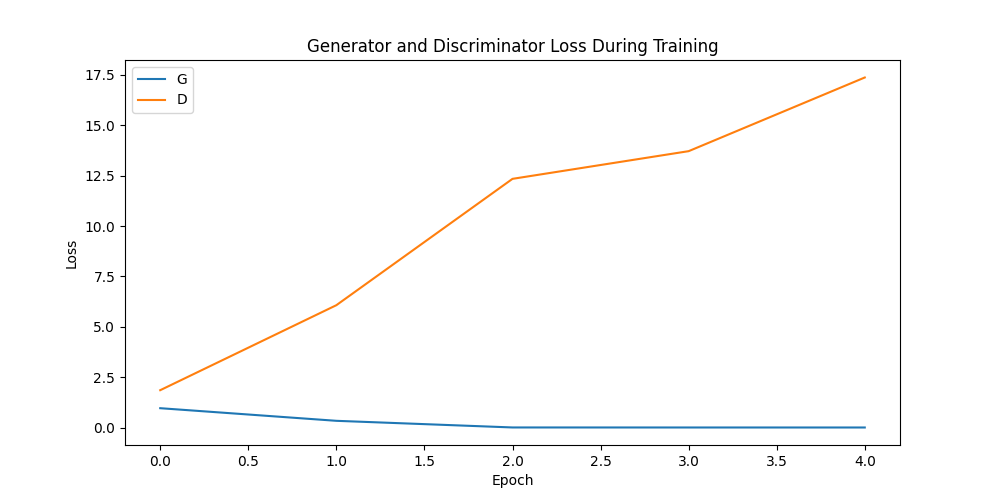
\includegraphics[width=0.8\textwidth]{gagan_loss_plot.png}
\caption{Generator and Discriminator Loss During Training.}
\label{fig:loss_curve}
\end{figure}


\subsection{Runtime \& Complexity}
\textbf{Theoretical Complexity:}
\begin{itemize}
    \item Generator training: $O(n)$ per batch
    \item Discriminator fitness evaluation: $O(p)$ per batch, where $p$ is population size
\end{itemize}

\textbf{Empirical Performance:}
\begin{itemize}
    \item Training on 10\% of CelebA with batch size 32, population 10 took approximately 5 minutes per epoch on CPU.
\end{itemize}

\begin{figure}[h!]
\centering
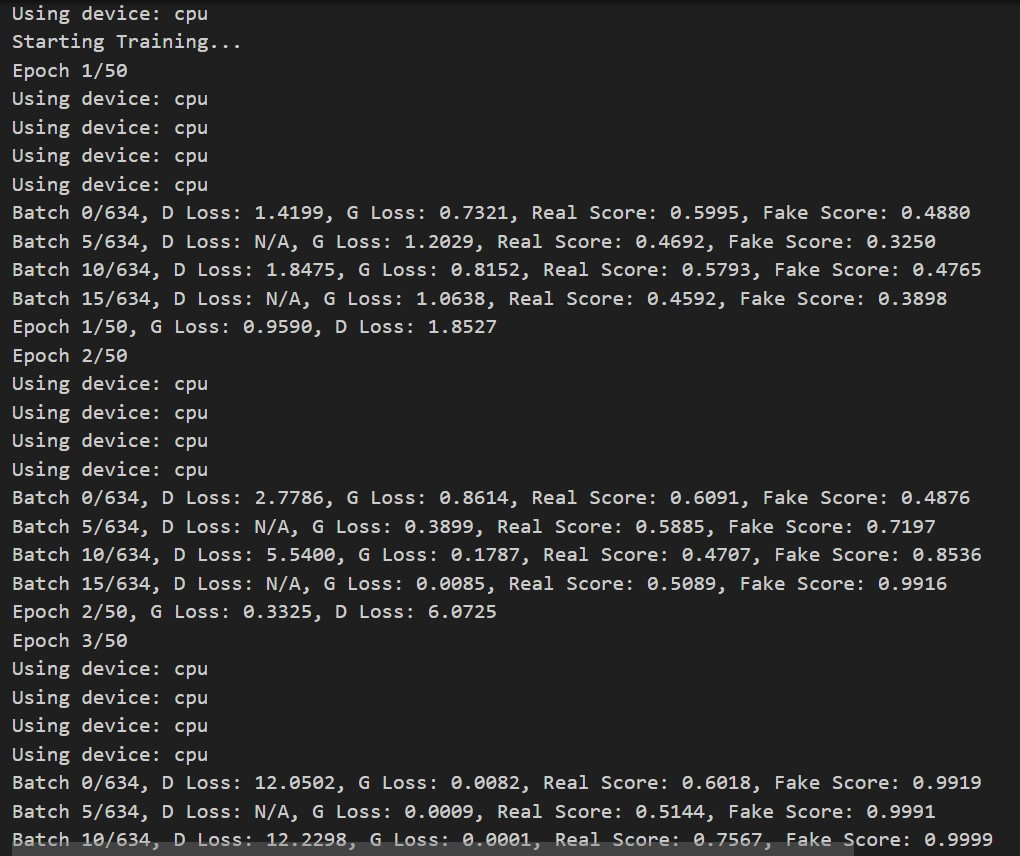
\includegraphics[width=0.8\textwidth]{tracking_progress.jpg}
\caption{Console outputs when training starts}
\label{fig:training_logs}
\end{figure}


\subsection{Comparisons}
\begin{center}
\begin{tabular}{|c|c|c|c|}
\hline
\textbf{Method} & \textbf{Training Stability} & \textbf{Output Diversity} & \textbf{Runtime} \\
\hline
Standard GAN & Poor & Limited & Fast \\
GAGAN        & Improved & High & Slower \\
\hline
\end{tabular}
\end{center}

\begin{figure}[h!]
\centering
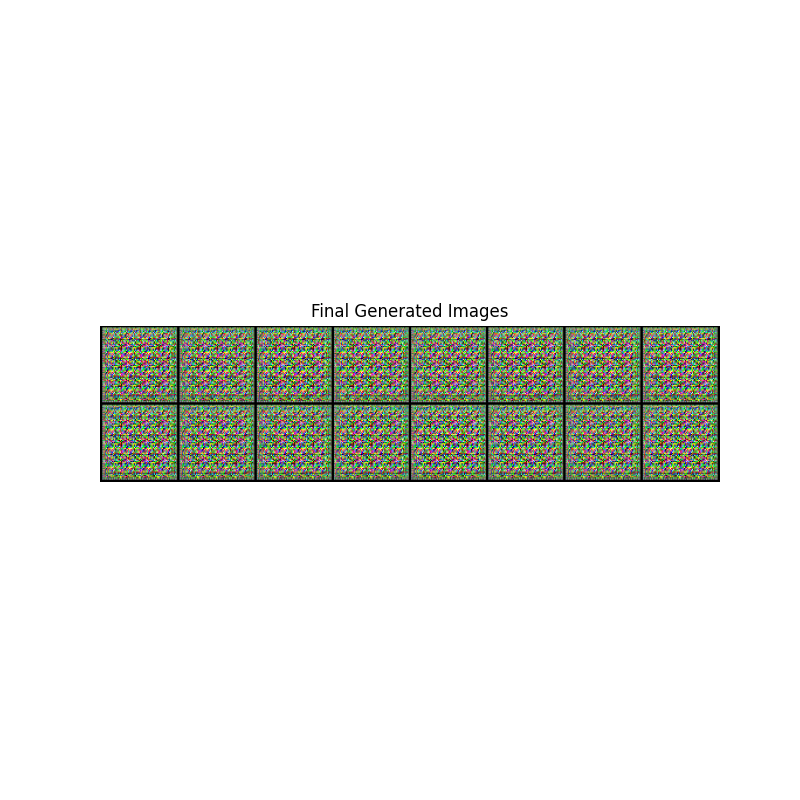
\includegraphics[width=0.8\textwidth]{final_generated_images.png}
\caption{Final Generated Images after Training GAGAN.}
\label{fig:final_generated}
\end{figure}


\subsection{Enhancements}
\begin{itemize}
    \item \textbf{Label Smoothing \& Noise Injection:} Improved training stability.
    \item \textbf{Real-World Dataset:} Used CelebA face dataset.
    \item \textbf{Hyperparameter Tuning:} Experimented with mutation rates, elite ratios, population sizes.
    \item \textbf{Visualization:} Regular loss plots and generated image snapshots.
\end{itemize}

\textbf{Impact:}
\begin{itemize}
    \item Better generator stability.
    \item Maintained discriminator diversity during evolution.
    \item Visual improvement in generated samples across epochs.
\end{itemize}

\section{Reflection}
\textbf{Challenges:}
\begin{itemize}
    \item Tuning genetic algorithm parameters without destabilizing training.
    \item Running evolutionary GANs without access to GPU for final tests.
\end{itemize}

\textbf{Learning Outcomes:}
\begin{itemize}
    \item Deepened understanding of GAN training dynamics.
    \item Gained practical experience in evolutionary computation for deep learning.
\end{itemize}

\textbf{Future Work:}
\begin{itemize}
    \item Implement hybrid models combining EA and backpropagation.
    \item Add spectral normalization and gradient penalties.
    \item Scale to larger datasets and higher resolutions.
    \item Parallelize genetic evolution to improve runtime.
\end{itemize}

\end{document}
